\clearpage
\phantomsection

\setcounter{chapter}{0}
\chapter[{Cơ sở lý thuyết}]{Cơ sở lý thuyết}

Chương này xây dựng nền tảng lý thuyết cần thiết để hiểu thiết kế và thực nghiệm của đề tài. Các phần dưới đây trình bày cơ chế hoạt động của từng kỹ thuật, những điểm cần lưu ý trong bối cảnh Roguelike và cách các kỹ thuật được dùng trong thực nghiệm.

\section{Game Action Roguelike và đặc trưng bài toán}

\textbf{Đặc trưng của thể loại.} Roguelike là thể loại game có bản đồ sinh ngẫu nhiên, độ khó cao và không có checkpoint. Biến thể Action Roguelike (ví dụ: \textit{Enter the Gungeon}, \textit{Hades}) thay thế lượt đi tuần tự bằng chiến đấu thời gian thực: nhân vật di chuyển và bắn súng liên tục trong khi né đạn của kẻ địch, tương tác với vật thể và phòng có bố cục khác nhau mỗi lần chơi. Thể loại này thách thức hơn game có bản đồ cố định vì tác nhân không thể ghi nhớ đường đi; thay vào đó cần học các quy tắc tổng quát.

\textbf{Tại sao đây là bài toán khó cho RL.} Môi trường của đề tài kết hợp ba thách thức đồng thời; mỗi thách thức đều có thể gây khó khăn đáng kể khi xét riêng lẻ:

\begin{itemize}
    \item \textbf{Phân phối bản đồ thay đổi:} mỗi episode dùng một bản đồ PCGNN khác nhau, làm phân phối dữ liệu quan sát thay đổi liên tục. Tác nhân phải khái quát hóa, không thể chỉ ghi nhớ bố cục.
    \item \textbf{Không gian hành động đa nhánh $(3,3,3,9)$:} tác nhân phải phối hợp đồng thời hướng di chuyển, ý định chiến đấu và góc ngắm bắn trong thời gian thực.
    \item \textbf{Phần thưởng thưa và trễ:} tiêu diệt kẻ địch hay dọn phòng chỉ xảy ra sau khi hoàn thành chuỗi hành vi tiếp cận--né--căn hướng--tấn công. Trong giai đoạn đầu huấn luyện, tín hiệu phần thưởng quá thưa để dẫn dắt học hiệu quả.
\end{itemize}

\textbf{Quan sát và hành động trong đề tài.} Tác nhân sử dụng vector quan sát cấu trúc 207 chiều (thay vì ảnh pixel) để tiết kiệm chi phí tính toán, bao gồm thông tin về người chơi, kẻ địch, đạn và tường. Không gian hành động rời rạc nhiều nhánh $(3,3,3,9)$ biểu diễn điều khiển trục X, trục Y, ý định chiến đấu và hướng ngắm. Đây là lý do đề tài cần curriculum learning và các kỹ thuật khám phá thay vì chỉ dùng PPO đơn thuần.

\section{Học tăng cường và PPO}
\subsection{Mô hình MDP và vòng lặp học}

Học tăng cường (RL) mô hình hóa bài toán dưới dạng Quy trình Quyết định Markov $(S,A,P,R,\gamma)$: tác nhân quan sát trạng thái $s_t \in S$, chọn hành động $a_t \in A$, nhận phần thưởng $r_t = R(s_t, a_t)$ và chuyển sang trạng thái mới $s_{t+1}$ theo xác suất $P(s_{t+1}|s_t,a_t)$. Mục tiêu là tìm chính sách $\pi_\theta$ tối đa hóa tổng phần thưởng chiết khấu:
\begin{equation}
    J(\pi_\theta) = \mathbb{E}_{\tau \sim \pi_\theta}
    \left[\sum_{t=0}^{T}\gamma^t r_t\right].
\end{equation}

\begin{figure}[H]
    \centering
    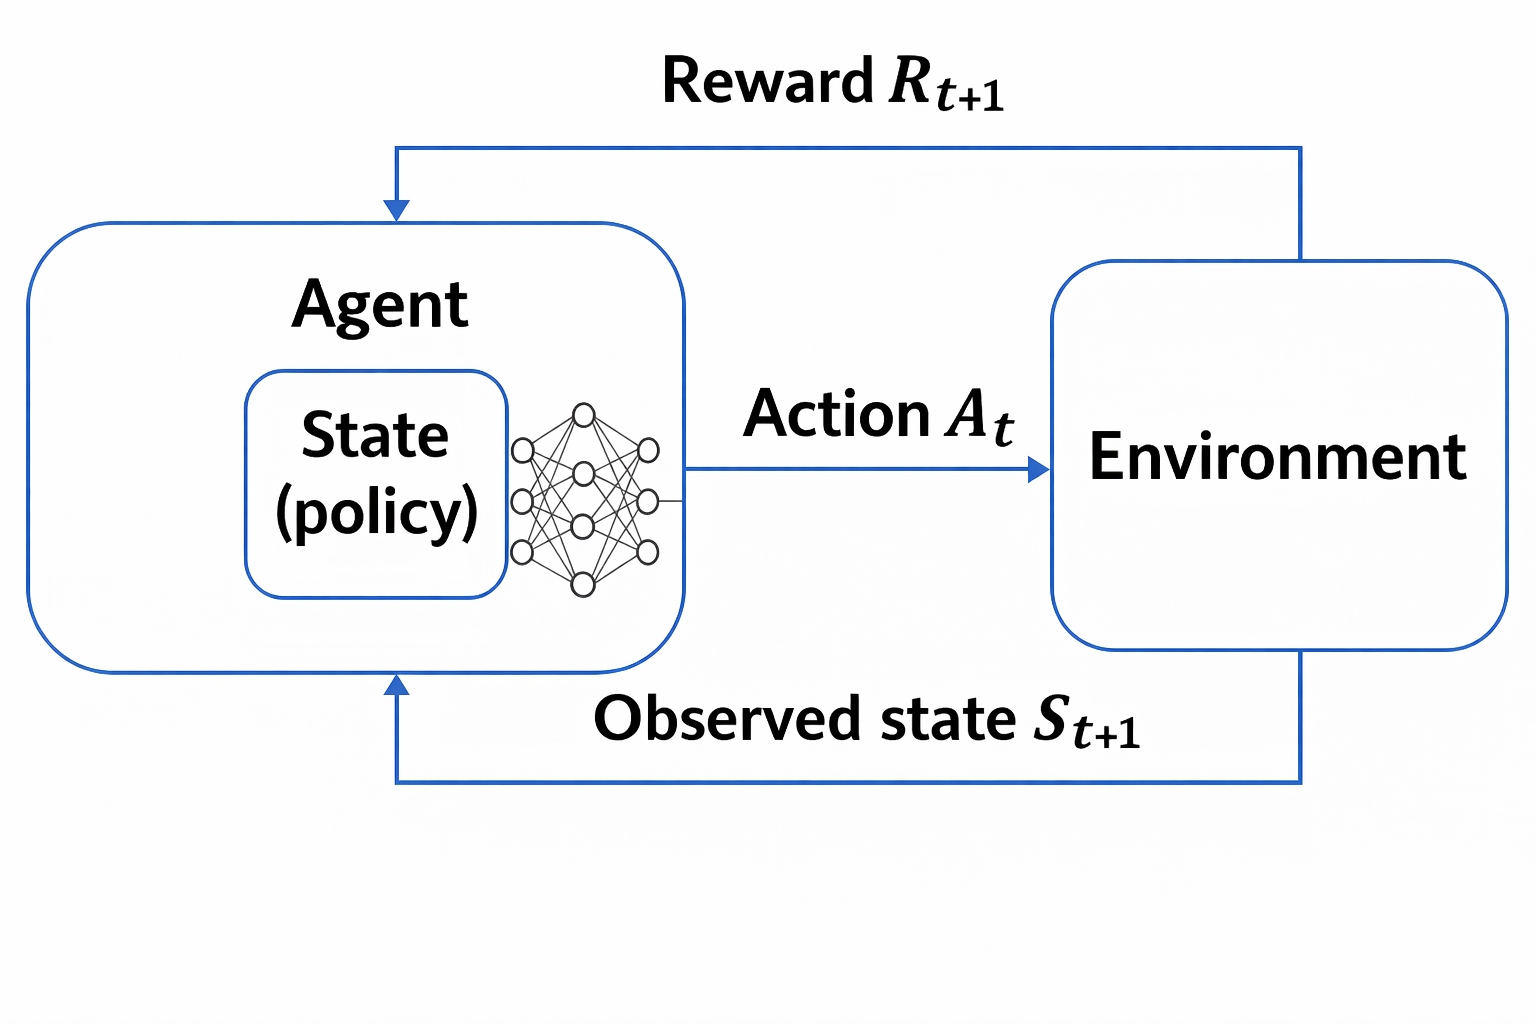
\includegraphics[width=0.9\linewidth]{figures/RL_Loop.png}
    \caption{Chu trình tương tác giữa tác nhân và môi trường trong học tăng cường.}
    \label{fig:rl_loop}
\end{figure}

Tác nhân không có dữ liệu có sẵn mà tự sinh dữ liệu qua tương tác, tạo ra ba khó khăn điển hình: khám phá vs. khai thác, phần thưởng trễ và tương quan thời gian giữa các mẫu.

\subsection{Proximal Policy Optimization (PPO)}

PPO được chọn làm thuật toán nền tảng vì hỗ trợ tốt không gian hành động rời rạc nhiều nhánh trong Unity ML-Agents và có độ ổn định cao \cite{Schulman2017}. PPO dùng kiến trúc Actor-Critic: Actor sinh phân phối xác suất $\pi_\theta(a|s)$, Critic ước lượng $V_\psi(s)$ làm baseline.

\begin{figure}[H]
\centering
\begin{tikzpicture}[
  box/.style={draw, rounded corners=3pt, minimum width=2.5cm, minimum height=0.8cm, align=center, font=\small},
  >=stealth
]
\node[box, fill=gray!15] (s)  at (0,0)     {Trạng thái $s_t$};
\node[box, fill=blue!12] (sh) at (4.0,0)   {Bộ trích đặc\\trưng chung};
\node[box, fill=orange!20] (ac) at (8.0, 1.1)  {Actor\\$\pi_\theta(a|s)$};
\node[box, fill=green!15]  (cr) at (8.0,-1.1)  {Critic\\$V_\psi(s)$};
\node[box, fill=orange!30] (a)  at (12.0, 1.1) {Hành động $a_t$};
\node[box, fill=green!25]  (v)  at (12.0,-1.1) {Giá trị $V(s_t)$};
\draw[->] (s) -- (sh);
\draw[->] (sh.north east) -- (ac.west);
\draw[->] (sh.south east) -- (cr.west);
\draw[->] (ac) -- (a);
\draw[->] (cr) -- (v);
\end{tikzpicture}
\caption{Kiến trúc Actor-Critic: Actor và Critic chia sẻ bộ trích đặc trưng, sau đó phân nhánh để sinh hành động và ước lượng giá trị.}
\label{fig:actor_critic}
\end{figure}

PPO giới hạn mức thay đổi chính sách qua tỷ lệ xác suất $\rho_t(\theta) = \pi_\theta(a_t|s_t) / \pi_{\theta_\text{old}}(a_t|s_t)$ và hàm mục tiêu có cắt ngưỡng:

\begin{equation} \label{eq:ppo_clip}
    L^{CLIP}(\theta) =
    \hat{\mathbb{E}}_t
    \left[
    \min
    \left(
    \rho_t(\theta)\hat{A}_t,\;
    \mathrm{clip}(\rho_t(\theta),1-\epsilon,1+\epsilon)\hat{A}_t
    \right)
    \right].
\end{equation}

Hàm mục tiêu tổng hợp kết hợp policy loss (mất mát chính sách), value loss (mất mát giá trị) và entropy bonus (thành phần thưởng entropy):
\begin{equation} \label{eq:ppo_total}
    L_t(\theta) = L_t^{CLIP}(\theta) - c_1 L_t^{VF}(\theta) + c_2 S[\pi_\theta](s_t).
\end{equation}

Thành phần entropy $S[\pi_\theta]$ đặc biệt quan trọng trong đề tài vì action space $(3,3,3,9)$ có tối đa 5.49 nat. Nếu entropy giảm quá sớm, tác nhân có thể hội tụ vào hành vi đơn điệu.

\subsection{Hàm lợi thế và GAE}

Hàm lợi thế $A(s_t,a_t) = Q(s_t,a_t) - V(s_t)$ cho biết hành động tốt hơn hay kém hơn kỳ vọng. PPO dùng Generalized Advantage Estimation (GAE) để ước lượng ổn định hơn:
\begin{equation}
    \delta_t = r_t + \gamma V(s_{t+1}) - V(s_t),
    \qquad
    \hat{A}_t^{GAE} = \sum_{l=0}^{T-t-1}(\gamma\lambda)^l \delta_{t+l}.
\end{equation}
Tham số $\lambda \in [0,1]$ điều chỉnh cân bằng giữa độ lệch và phương sai. Trong môi trường của đề tài có cả phần thưởng định hình dày đặc và phần thưởng kết quả thưa, GAE giúp ổn định tín hiệu học.

\section{Các kỹ thuật hỗ trợ}

\subsection{Intrinsic Curiosity Module (ICM)}

ICM bổ sung phần thưởng nội tại $r_t^{int}$ dựa trên sai số dự đoán chuyển trạng thái \cite{Pathak2017}. ICM huấn luyện hai mô hình phụ trên không gian đặc trưng $\phi(s)$: inverse model dự đoán $a_t$ từ $(\phi(s_t), \phi(s_{t+1}))$, và forward model dự đoán $\hat{\phi}(s_{t+1})$ từ $(\phi(s_t), a_t)$. Sai số forward model trở thành phần thưởng khám phá:
\begin{equation}
    r_t^{ICM} = \tfrac{1}{2}\|\hat{\phi}(s_{t+1}) - \phi(s_{t+1})\|_2^2, \qquad
    L_{inv} = CE(a_t,\, g(\phi(s_t),\phi(s_{t+1}))).
\end{equation}

\begin{figure}[H]
    \centering
    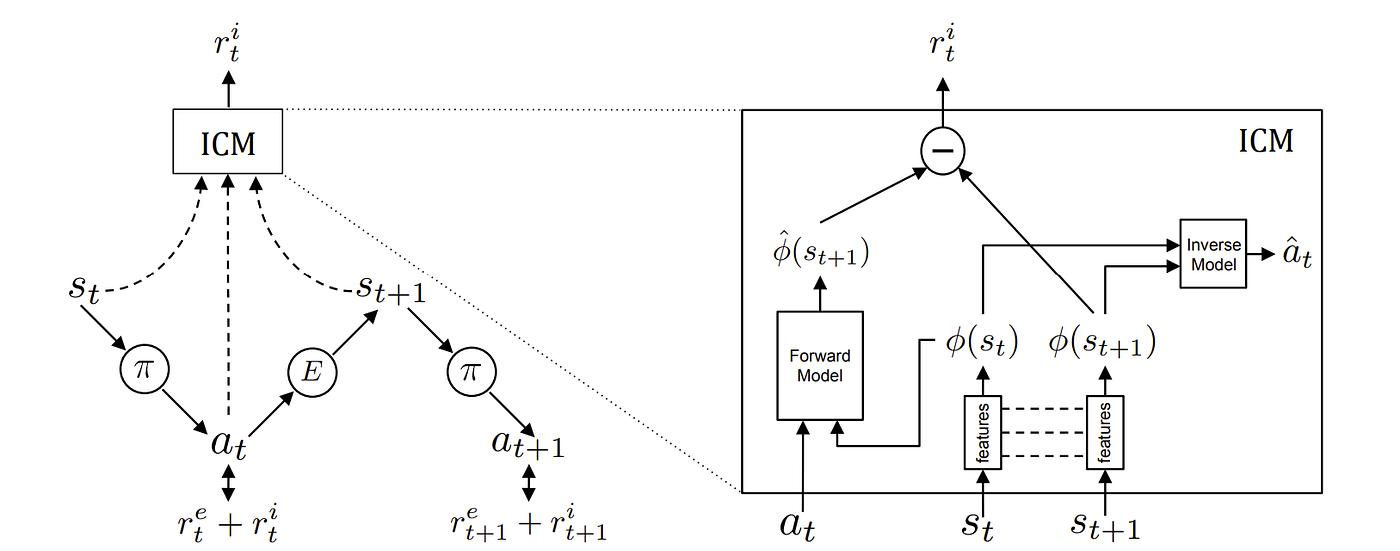
\includegraphics[width=\textwidth]{figures/icm.png}
    \caption{Mô hình ICM: inverse model và forward model sinh phần thưởng nội tại dựa trên sai số dự đoán chuyển trạng thái.}
    \label{fig:icm_original}
\end{figure}

Trong bài toán của đề tài, inverse model cần học quan hệ giữa chuyển trạng thái và tổ hợp hành động $(3,3,3,9)$. Không gian hành động đa nhánh này làm bài toán dự đoán hành động khó hơn, vì nhiều nhánh hành động có thể cùng ảnh hưởng đến kết quả chuyển trạng thái. Nếu inverse loss không giảm đủ và vẫn gần entropy ngẫu nhiên 5.49 nat, ICM khó khuyến khích đúng các chuyển tiếp hữu ích cho chiến đấu. Kết quả Chương~4 xác nhận inverse loss dừng ở 4.36 nat.

Trong thực nghiệm, ICM được kết hợp với curriculum learning trong run50 để hai kỹ thuật bổ trợ cho nhau: curriculum tạo tín hiệu học sớm, còn ICM tăng cường khám phá trong từng lesson.

\subsection{Random Network Distillation (RND)}

RND dùng hai mạng: mạng mục tiêu $f$ (cố định, ngẫu nhiên) và mạng dự đoán $\hat{f}_\theta$ (học). Phần thưởng nội tại là sai số bắt chước \cite{Burda2018}:
\begin{equation}
    r_t^{RND} = \|\hat{f}_\theta(s_t) - f(s_t)\|_2^2.
\end{equation}
Trạng thái ít gặp → sai số cao → phần thưởng cao. Khi trạng thái được thăm nhiều, sai số tự giảm.

RND thưởng cho trạng thái mới lạ bất kể có liên quan đến chiến đấu hay không. Trong môi trường có tường phức tạp, tác nhân có thể khám phá góc phòng thay vì học tiếp cận kẻ địch. Do không có thành phần phụ thuộc hành động, tín hiệu RND không phản ánh trực tiếp tính hữu ích của từng chuyển tiếp đối với chiến đấu.

Trong thực nghiệm, RND được so sánh trực tiếp với ICM qua ablation (run35 vs run36) để xác định kiểu khám phá nào phù hợp hơn với môi trường Roguelike chiến đấu.

\subsection{Bộ nhớ LSTM}

LSTM duy trì trạng thái ẩn $h_t$ và cell $c_t$ qua các bước thời gian \cite{Hochreiter1997}, cho phép tích lũy thông tin lịch sử mà MLP thuần túy không có. Cơ chế cổng (forget, input, output) kiểm soát có chọn lọc thông tin nào được giữ hay xóa.

Thêm LSTM làm tăng chi phí tính toán và thường làm chậm hội tụ ban đầu. Quan trọng hơn, nếu quan sát đã đủ thông tin (ví dụ trạng thái hiện tại đã bao gồm cooldown, velocity, hướng kẻ địch), mức cải thiện từ bộ nhớ tuần tự có thể không đủ để bù chi phí tính toán. Đây là giả thuyết cần kiểm tra bằng ablation.

Để kiểm tra giả thuyết này, run42 (PPO+LSTM) và run47 (Curriculum+LSTM) được so sánh với các run tương ứng không dùng LSTM. Kết quả Chương~4 cho thấy LSTM học chậm hơn nhưng không tạo ra cải thiện rõ rệt khi sử dụng riêng lẻ.

\subsection{PCGNN và sinh bản đồ bằng neuroevolution}

PCGNN (Procedural Content Generation using NEAT and novelty search) tiến hóa một mạng nơ-ron $f_\theta$ sinh bản đồ tile-by-tile \cite{Beukman2022}. Mỗi ô $(i,j)$ được sinh bởi:
\begin{equation}
    t_{i,j} = \arg\max\, f_\theta(C(i,j),\, \mathbf{z}),
\end{equation}
trong đó $C(i,j)$ là ngữ cảnh lân cận $3\times3$ và $\mathbf{z}$ là nhiễu ngẫu nhiên để tạo đa dạng. Quá trình tiến hóa dùng novelty search để tránh hội tụ sớm về một mẫu bản đồ duy nhất.

Bản đồ được đánh giá bằng bốn chỉ số thường dùng trong PCGNN: \textbf{Leniency} (tỷ lệ sàn), \textbf{A* Difficulty} (độ phức tạp đường đi), \textbf{Compression Distance} (độ khác biệt cấu trúc giữa các bản đồ) và \textbf{A* Diversity} (phương sai độ khó trong cùng một genome).

PCGNN hướng tới bài toán mê cung (maze), tối ưu hóa khả năng giải và tìm đường. Đối với Roguelike chiến đấu, cần thêm điều kiện: (1) tồn tại đường đi BFS giữa vị trí người chơi và kẻ địch, (2) không gian chiến đấu đủ rộng để di chuyển và né đạn, (3) phân phối độ khó phù hợp với curriculum.

Dựa trên PCGNN, đề tài thực hiện ba điều chỉnh gồm: (1) thêm bộ kiểm tra BFS để loại các bản đồ không bảo đảm tương tác chiến đấu hợp lệ giữa người chơi và kẻ địch, (2) bổ sung \texttt{dead\_end\_ratio}, \texttt{reachable\_ratio} và \texttt{difficulty\_score} vào tiêu chí tuyển chọn, (3) dùng PCGNN như bước tiền xử lý ngoại tuyến (offline) thay vì tích hợp trực tiếp vào vòng lặp huấn luyện để tránh rủi ro tích hợp Python--Unity. Chi tiết ở Chương~2--3.

\subsection{Curriculum Learning}

Curriculum learning tổ chức quá trình học từ dễ đến khó \cite{Bengio2009}. Tác nhân bắt đầu từ bản đồ Easy, chuyển sang Medium rồi Hard khi đạt ngưỡng hiệu quả. Điều kiện chuyển lesson dùng trung bình trượt EMA:
\begin{equation}
    \bar{G}_t = (1-\alpha)\bar{G}_{t-1} + \alpha G_t.
    \label{eq:curriculum_ema}
\end{equation}
Khi $\bar{G}_t \geq \theta_\ell$, trainer tăng tham số \texttt{difficulty}, từ đó kích hoạt TilemapGenerator chuyển sang nhóm bản đồ tương ứng.

Ngưỡng chuyển lesson $\theta_\ell$ cần được chỉnh tay theo từng môi trường, do chưa có cơ chế tự động điều chỉnh. Nếu ngưỡng quá thấp, tác nhân chuyển sang Hard quá sớm trước khi học xong kỹ năng cơ bản; nếu quá cao, tác nhân bị giữ lại ở Easy quá lâu.

Trong đề tài, ngưỡng được chỉnh thực nghiệm qua các run trước khi thiết kế ma trận ablation chính. Curriculum gắn trực tiếp với PCGNN: bản đồ được chia thành Easy/Medium/Hard theo percentile trước khi đưa vào TilemapGenerator. Kết quả Chương~4 cho thấy đây là kỹ thuật có ảnh hưởng lớn nhất, +85\% so với PPO baseline.

\section{Tóm tắt chương}

Chương này trình bày nền tảng RL (MDP, PPO, GAE), đặc trưng của Roguelike chiến đấu và năm kỹ thuật hỗ trợ (ICM, RND, LSTM, PCGNN, curriculum) kèm phân tích hạn chế và cách đề tài điều chỉnh. Bảng~\ref{tab:technique_summary} tóm tắt mối liên hệ giữa các kỹ thuật này với mục tiêu của đề tài.

\begin{table}[H]
    \centering
    \small
    \caption{Tổng hợp kỹ thuật và mục tiêu đề tài}
    \label{tab:technique_summary}
    \begin{tabular}{|l|l|l|p{4.5cm}|}
        \hline
        \textbf{Kỹ thuật} & \textbf{Mục tiêu} & \textbf{Hạn chế chính} & \textbf{Cách đề tài xử lý} \\
        \hline
        PPO & chiến đấu & Cần nhiều bước để hội tụ trong môi trường có phần thưởng thưa & Kết hợp với curriculum \\
        \hline
        ICM & so sánh kỹ thuật & Inverse model khó với không gian hành động $(3,3,3,9)$ & Ablation run35, run50 \\
        \hline
        RND & so sánh kỹ thuật & Thưởng trạng thái mới không liên quan chiến đấu & Ablation run36 \\
        \hline
        LSTM & so sánh kỹ thuật & Học chậm, có thể không cần nếu quan sát đã đủ thông tin & Ablation run42, run47 \\
        \hline
        PCGNN & curriculum/bản đồ & Thiết kế cho mê cung, chưa trực tiếp phục vụ chiến đấu & Điều chỉnh fitness và kiểm tra BFS \\
        \hline
        Curriculum & curriculum/bản đồ & Ngưỡng chuyển lesson cần chỉnh tay & Chỉnh thực nghiệm + EMA \\
        \hline
    \end{tabular}
\end{table}

Chương~2 sẽ mô tả cách các thành phần trên được tích hợp thành hệ thống hoàn chỉnh, bắt đầu bằng tổng quan pipeline end-to-end trước khi đặc tả từng phần.
